\section{Results}
\label{sec:bench}

\subsection{Method}
We run all our experiments on Cloudlab [5] xl170 machine, with a ten-core Intel E5-2640v4 running at 2.4 GHz, 64GB ECC Memory (4x 16 GB DDR4-2400 DIMMs), Intel DC S3520 480 GB 6G SATA SSD and 10Gbps NIC. We run on Ubuntu 18.04 (4.15.0-55-generic). We performed all the experiments on Postgresql version 10.10 and SQLite3 version 3.22.0. Postgres was configured to run with a  single thread by changing \texttt{max\_parallel\_workers} = 1, \texttt{max\_worker\_processes} = 1 and \texttt{max\_parallel\\\_workers\_per\_gather} = 0. The buffer pool for each system was set to 20MB.

We first measure the execution times for both the benchmarks and then compare the query plans generated for few queries from TPCH to understand the difference in execution time. 


\subsection{Execution Time}
\label{sec:time}

\fig{width=\columnwidth}{tpch_result}{\textmd{TPCH result}}{fig:tpch_result}
\fig{width=\columnwidth}{ssb_result}{\textmd{SSB result}}{fig:ssb_result}


The total execution time for TPCH is shown in Figure~\ref{fig:tpch_result}. We observe that postgres is not always faster, sqlite is competitive in some cases. The same behaviour is observed for SSB in Figure~\ref{fig:ssb_result}. These results give us an overall picture of the execution time of one system in comparison with the other.
. 


\subsection{Query Plan Comparison}
\label{sec:plan}

\subsubsection{Almost same time}
\fig{width=\columnwidth}{tpch-postgres-16}{\textmd{Postgres plan for query 16}}{fig:tpch-postgres-16}

\begin{figure*}[ht]
\centering
     \begin{subfigure}[b]{0.4\textwidth}
         \centering
         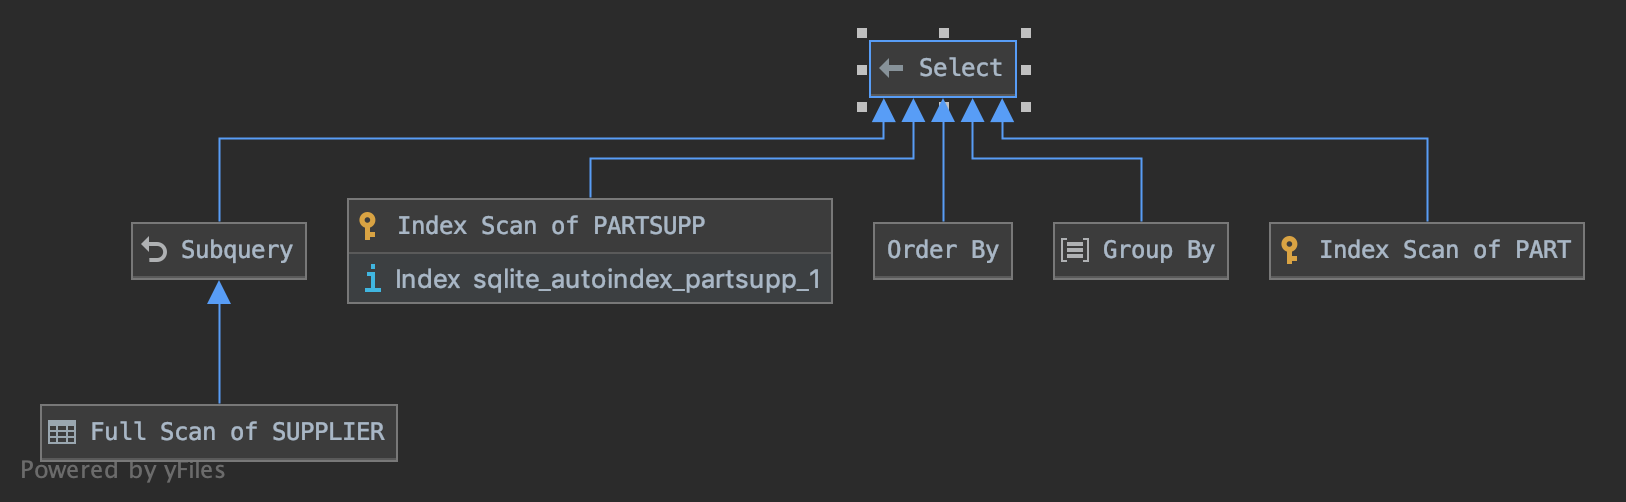
\includegraphics[width=\columnwidth]{tpch-sqllite-16}
         \caption{SQLite query plan 16 steps}
         \label{fig:tpch-sqllite-16}
     \end{subfigure}
     \hfill
     \begin{subfigure}[b]{0.4\textwidth}
         \centering
         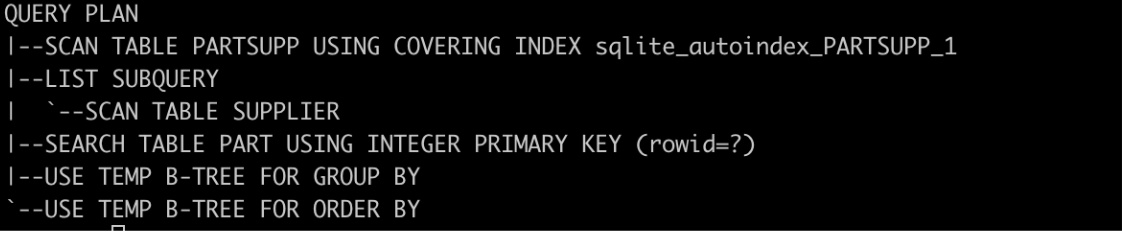
\includegraphics[width=\columnwidth]{sqlite-16-2}
         \caption{SQLite query plan 16}
         \label{fig:sqlite-16-2}
     \end{subfigure}

        \caption{SQLite plan for query 16}
        \label{fig:sqlite-16}
\end{figure*}

We now look at query 16 represented in Listing~\ref{q16} from the TPCH benchmark suite. In this query is the Parts/Supplier Relationship Query that returns how many suppliers can supply parts with given attributes. This query has almost same time for both, postgres and sqlite. 

Figure~\ref{fig:tpch-postgres-16} shows the query plan generated for this query in postgres, we observe that it does a full scan of all the tables followed by some hash joins, sort, aggregate and then sort again. If we look at the query plan for SQLite in Figure~\ref{fig:sqlite-16}, we observe that it also does a scan of all the tables and execute a similar query plan. Since the query plans generated by both are significantly similar and this query does not contain the big table, LINEITEM, therefore the scans take similar time even though SQLite does an index scan. All this add up to almost same time for this particular query in both the databases.\\

\begin{minipage}{\linewidth}
\begin{lstlisting}[breaklines=true, numbers=none, label=q16, caption=Query 16]
select p_brand, p_type, p_size, count(distinct ps_suppkey) as supplier_cnt
from
partsupp, part
where
p_partkey = ps_partkey
and p_brand <> '[BRAND]'
and p_type not like '[TYPE]%'
and p_size in ([SIZE1], [SIZE2], [SIZE3], [SIZE4], [SIZE5], [SIZE6], [SIZE7], [SIZE8])
and ps_suppkey not in (
select s_suppkey
from supplier
where
s_comment like '%Customer%Complaints%'
)
group by p_brand, p_type, p_size
order by
supplier_cnt desc,
p_brand,
p_type,
p_size;;
\end{lstlisting}
\end{minipage}



%\fig{width=\columnwidth}{tpch-sqllite-16}{\textmd{TPCH result}}{fig:tpch-sqllite-16}



\subsubsection{Postgres faster}
\fig{width=\columnwidth}{tpch-postgres-9}{\textmd{Postgres plan for query 9}}{fig:tpch-postgres-9}

\begin{figure*}[ht]
\centering
     \begin{subfigure}[b]{0.4\textwidth}
         \centering
         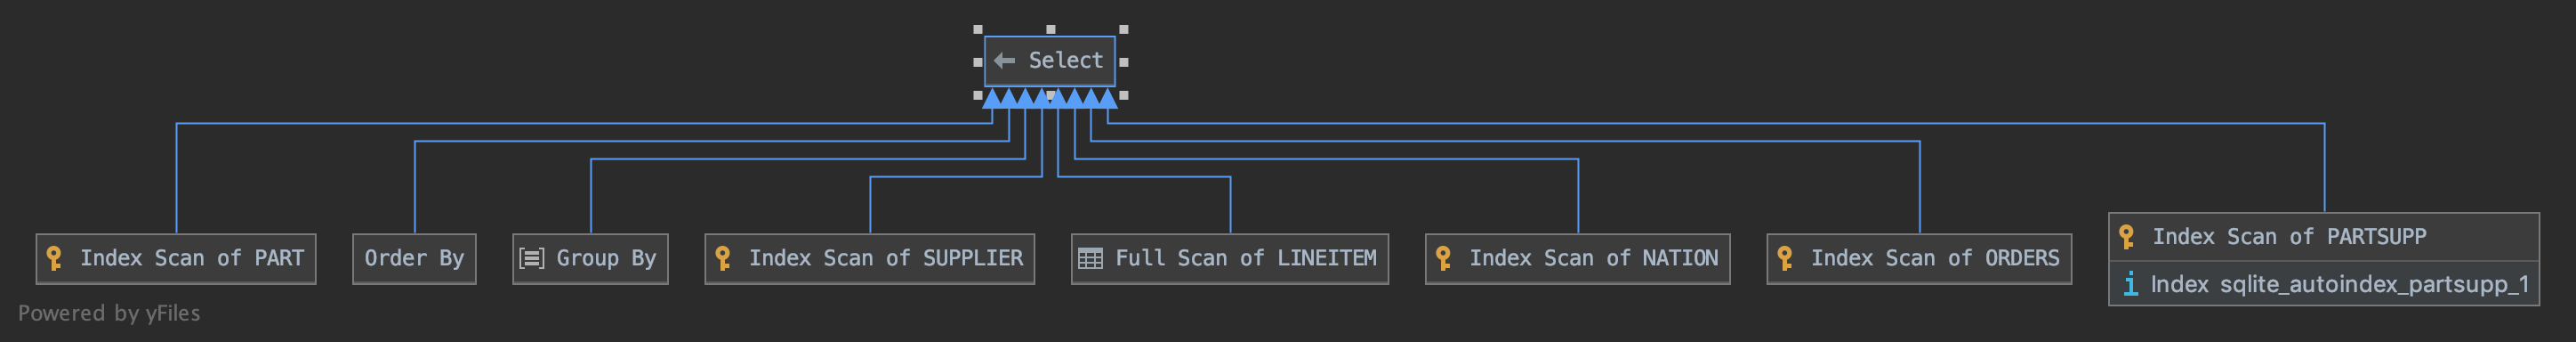
\includegraphics[width=\columnwidth]{tpch-sqllite-9}
         \caption{SQLite query plan 9 steps}
         \label{fig:tpch-sqllite-9}
     \end{subfigure}
     \hfill
     \begin{subfigure}[b]{0.4\textwidth}
         \centering
         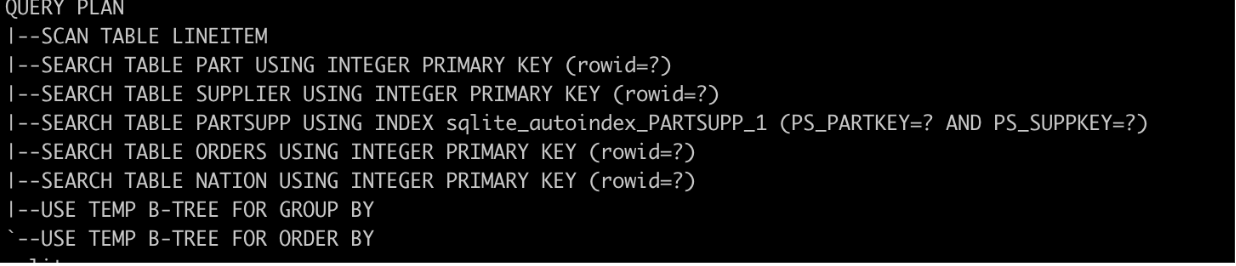
\includegraphics[width=\columnwidth]{sqlite-9-2}
         \caption{SQLite query plan 9}
         \label{fig:sqlite-9-2}
     \end{subfigure}

        \caption{SQLite plan for query 9}
        \label{fig:sqlite-9}
\end{figure*}
%\fig{width=\columnwidth}{tpch-sqllite-9}{\textmd{TPCH result}}{fig:tpch-sqllite-9}
Query 9 shown in Listing~\ref{q9} called Product Type Profit Measure Query which determines how much profit is made on a given line of parts, broken out by supplier nation and year. This query takes longer execution time SQLite.

Figure~\ref{fig:tpch-postgres-9} shows the query plan for Postgres where we observe that it does full scan of all the tables followed by hash join and aggregate at the end. In SQLite shown in Figure~\ref{fig:sqlite-9}, we see many index scans. We also see that this query has LINEITEM which is a big table and hence, selectively for this particular query is very high. Therefore, index scan in this scan becomes expensive over full scan which is seen by the lower execution time for Postgres.

\begin{minipage}{\linewidth}
\begin{lstlisting}[breaklines=true, numbers=none, label=q9, caption=Query 9]
select nation, o_year, sum(amount) as sum_profit
from (
select
n_name as nation,
extract(year from o_orderdate) as o_year,
l_extendedprice * (1 - l_discount) - ps_supplycost * l_quantity as amount
from part, supplier, lineitem, partsupp, orders, nation
where
s_suppkey = l_suppkey
and ps_suppkey = l_suppkey
and ps_partkey = l_partkey
and p_partkey = l_partkey
and o_orderkey = l_orderkey
and s_nationkey = n_nationkey
and p_name like '%[COLOR]%'
) as profit
group by
nation,
o_year
order by
nation,
o_year desc;
\end{lstlisting}
\end{minipage}

\subsubsection{SQLite faster}

\fig{width=\columnwidth}{tpch-postgres-4}{\textmd{Postgres plan for query 4}}{fig:pgsql-4}

\begin{figure*}[ht]
\centering
     \begin{subfigure}[b]{0.4\textwidth}
         \centering
         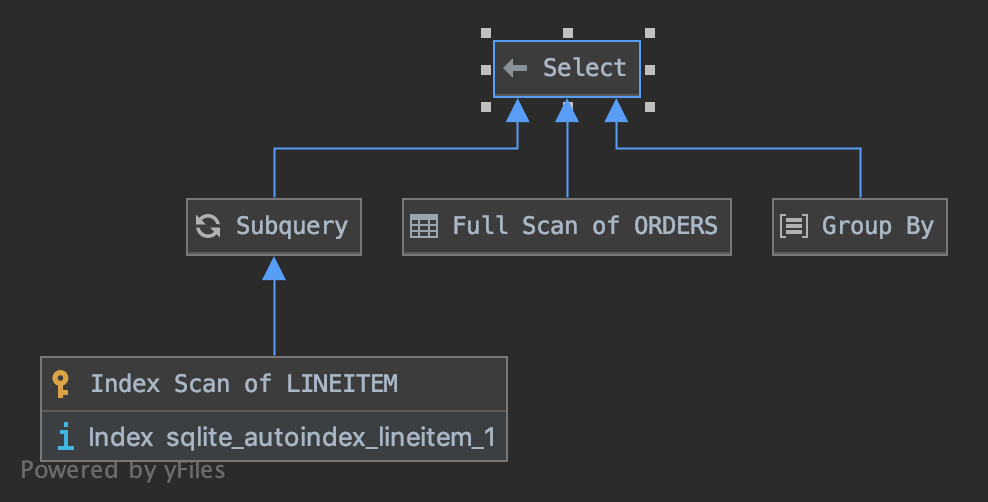
\includegraphics[width=\columnwidth]{tpch-sqllite-4}
         \caption{SQLite query plan 4 steps}
         \label{fig:tpch-sqllite-4}
     \end{subfigure}
     \hfill
     \begin{subfigure}[b]{0.4\textwidth}
         \centering
         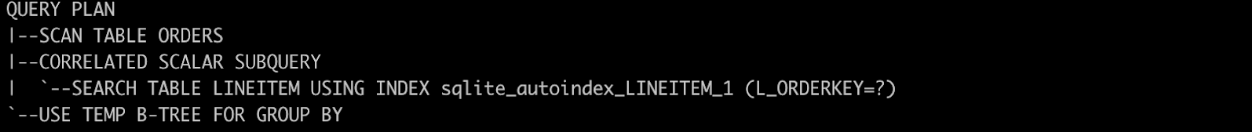
\includegraphics[width=\columnwidth]{sqlite-4-2}
         \caption{SQLite query plan 4}
         \label{fig:sqlite-4-2}
     \end{subfigure}

        \caption{SQLite plan for query 4}
        \label{fig:sqlite-4}
\end{figure*}
%\fig{width=\columnwidth}{tpch-sqllite-4}{\textmd{TPCH result}}{fig:tpch-sqllite-4}
Query 4 shown in Listing~\ref{q4} is called Order Priority Checking Query which finds how well the order priority system is working and gives an assessment of customer satisfaction. This query runs faster in SQLite.

The query plan for Postgres is shown in Figure~\ref{fig:pgsql-4} and SQLite is shown in Figure~\ref{fig:sqlite-4}. This query has an inner query which is called a correlated subquery~\cite{ref:sqlite1} which depends on the outer query. The selectively of this query is less that 5\%. In case of Postgres we observe  that it does a full scan of all the tables whereas SQLite uses an index scan. In queries where selectively is low, index scan is faster, therefore, we see that SQLite performs better than Postgres.

\begin{minipage}{\linewidth}
\begin{lstlisting}[breaklines=true, numbers=none, label=q4, caption=Query 4]
select o_orderpriority, count(*) as order_count
from
orders
where
o_orderdate >= date '[DATE]'
and o_orderdate < date '[DATE]' + interval '3' month
and exists (
select * from lineitem
where l_orderkey = o_orderkey and l_commitdate < l_receiptdate
)
group by o_orderpriority, order by, o_orderpriority;
\end{lstlisting}
\end{minipage}






